\begin{figure}[H]
    \centering
    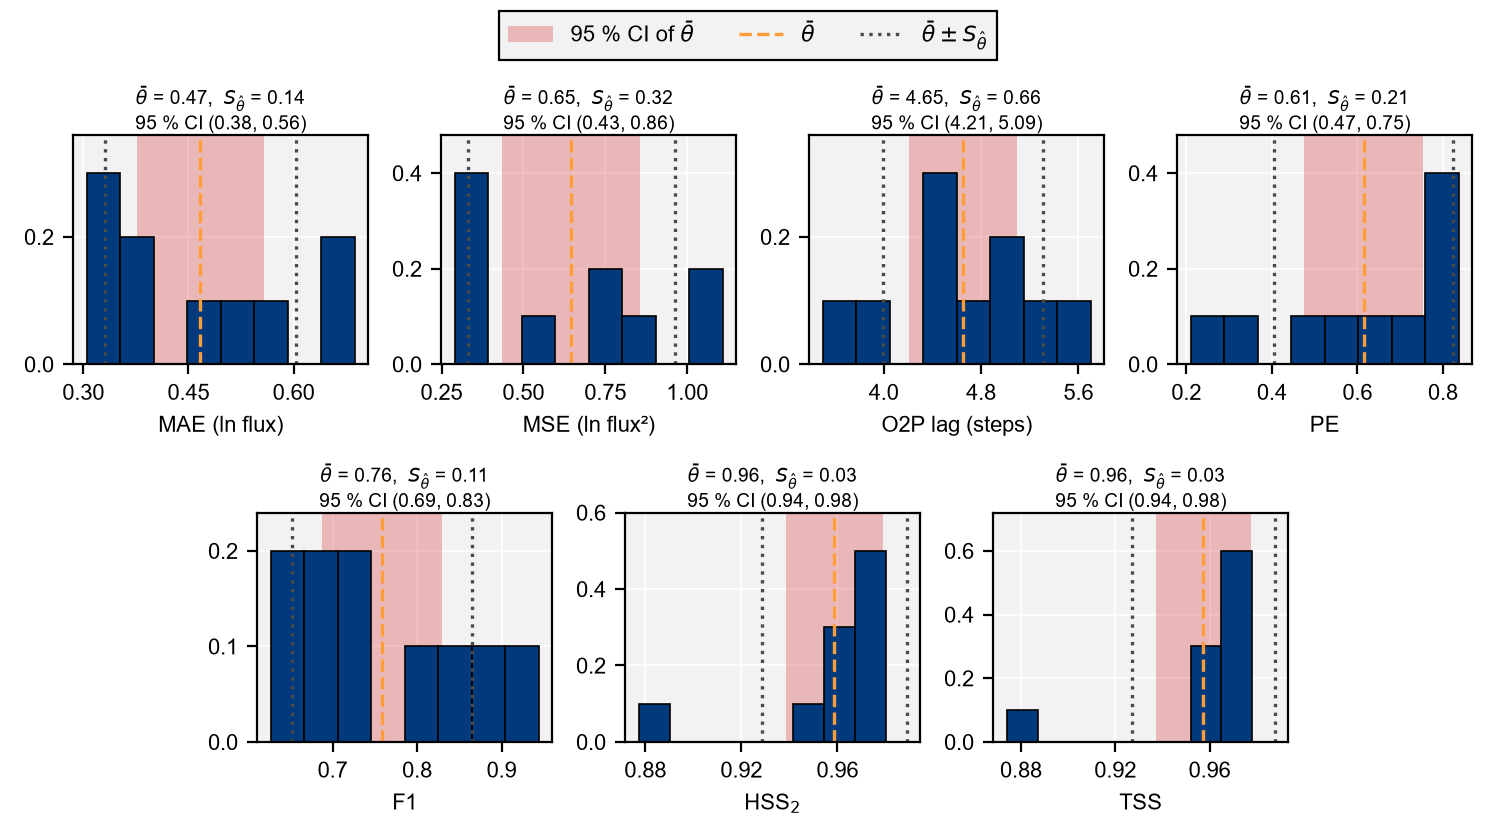
\includegraphics[width=\textwidth,height=0.55\textheight,keepaspectratio]{figs/evaluation/evaluation_of_sep_time_intensity_profile_prediction/resampled_time_series_block_bootstrapping/sin_metrics_t6_phases.png}
    \caption{Bootstrap distributions of the evaluation metrics for the sinusoidal transformer at the $t+6$ forecast horizon with phases, over the $B=10$ bootstrap datasets. Each panel shows the relative frequency of one metric: mean absolute error (MAE), mean squared error (MSE), onset-to-peak (O2P) lag, prediction efficiency (PE), F1, Heidke skill score (HSS$_2$), and true skill statistic (TSS). The orange dashed line is the mean $\bar{\theta}$, the dotted lines are $\bar{\theta} \pm S_{\hat{\theta}}$ , and the shaded region is the 95\% confidence interval of $\bar{\theta}$. The values of $\bar{\theta}, S_{\hat{\theta}}$ and the confidence interval are printed above each panel.}
    \label{fig:sin_metrics_t6_phases}
\end{figure}
